\chapter{The Readings}
% Covers: outline D1-D4: the coupling bracket; the balance; the calibration exhibit; the landing
% Chapter language (per Ch1 protocol): the geometry of frames (QED -> GR).
% The full frame story is owned by later sections; D4b/F3 material stays fenced, unspent.

\section{The flagship reading}
% Node-map: D1 whole -- the bracket ASSERTED ([129.6, 137.7], the walk's fences carried
% into the reading's units, exact ratios); the deep ~137.011 as DISPLAY per Ch1's
% protocol (turn-509 watch-item LANDS HERE, explicit not implied); the K5 fence
% displayed AS a fence at full strength; the three-pin falsifier attached in book
% language with the scope limit stated. ANNOTATION: NO rows land in S1 -- all six of
% the chapter's rows (EXP-9, EXP-3 fwd-ref, Archimedes, Cavendish, Unruh, Rindler)
% land in S2-S4, per map. Gate: turn 520 (Ch5 S1, ~1100 words).

This chapter speaks the geometry of frames, as the map announced, and the change of
language is the change of subject. For three chapters the instrument has been a
machine among machines --- rules, texts, transcripts. From here it is also an
observer: a thing that stands somewhere, and reads from where it stands. The full
story of where it stands, and of what kind of frame that is, belongs to later
sections and is not spent now. What matters first is the reading itself, because the
book has been walking toward this page since its first sentence.

The walk of the last chapter left two fences standing with the crossing pinned
between them: seventeen ninths below it, two above. One step remains: carry those
fences out of the walk's units and into the units a coupling is quoted in. The
instrument performs the carrying itself, in the same exact arithmetic as everything
else, and the conversion is no anonymous machine --- it has a shape the reader can
hold in one hand. It is a reciprocal. The coupling arrives as a measured ratio, and
the number the world quotes is that ratio turned over --- one over the measurement,
floored at the instrument's readout scale. The instrument reaches the reading in two
steps, the contraction from displacement to coupling and then the turn-over, and the
two steps compose to a single line the reader can work by hand: take the
displacement $d$, form $d/(d-1)$, and multiply by a fixed asymptote, $324/5$ ---
eighteen squared over five, and the reader has already met both of those numbers:
the eighteen is Chapter 4's measured slip, the five its floor-plus-one.

Now watch the fences go through, one at a time. The far fence stands at $2$: there
$d/(d-1)$ is $2$, and twice $324/5$ is $648/5$ --- $129.6$. The near fence stands at
$17/9$: there $d-1$ is $8/9$, so $d/(d-1)$ is $17/8$, and seventeen eighths of
$324/5$ is $1377/10$ --- $137.7$. Both walls are exact ratios of counts; the floor
in the machine's read bites nothing at either fence; the decimal points are a
courtesy only. And notice that the order crossed over: the fence below the crossing
landed as the wall above the reading, and the far fence as the low wall. That is the
reciprocal's signature --- $d/(d-1)$ falls as $d$ climbs --- and nothing about the
flip is left to prose: that the low wall stands below the high one is
machine-checked on every cold run, and that check is one of the falsifier's pins,
stated below.

So the two fences of the walk become the two walls of the reading --- the same two
boundaries, carried into the coupling's units and set to a new job: in the walk they
stopped an advance; here they hold an interval.

Here, then, is the flagship reading, stated as what this argument stands behind:

\begin{center}
$129.6 \;<\; \alpha^{-1}_{\mathrm{device}} \;<\; 137.7$
\end{center}

--- the inverse coupling, as this device measures it, lies between those walls. The
assertion is the interval, whole: two walls in proved order, three runs deep,
standing on three immune inputs, every number in the chain earned at a named site.
When this book is asked what it found, this is the answer. Nothing about the
sentence is provisional, and nothing about it is a point.

The reader will want the point anyway, and the book will show it --- under the
protocol Chapter 1 set, which lands here with its full weight. The fencepost stops
the assertion at three runs; it does not forbid watching the walk go on. Continued
past the stop, for display only, the walls keep closing, and they close toward a
value near $137.011$.

That number is on the page for the same reason a laboratory writes down where the
needle seems to rest: the reader wants to see it, and hiding it would be its own
dishonesty. Every real instrument is read this way. The graduation marks are the
assertion --- the needle lies between these two --- and the position between the
marks is the reader's interpolation. The book supplies the marks. The interpolated
value belongs to the reader's eye, and the instrument never signs it.

So the two numbers on this page differ in kind, not in degree, and the difference
is the book's entire epistemology in miniature. \emph{The bracket is asserted}:
three runs of earned count under it, and it dies if any one of them fails.
\emph{The deep value is displayed}: nothing under it but the reader's desire to
look further. The reading protocol said --- before the reader knew which number the
rule would protect --- that any single number quoted from an interval is a display
convenience, not an assertion. It protects this one.

And now the fence the whole book leans on, displayed as the flagship's own:

\begin{fence}
The value this instrument measures is its own. The laboratory's inverse coupling,
$137.036$, is not derived in this book, not matched, and not approached
asymptotically; no argument here bridges from the device's value to the
laboratory's. The two numbers are neighbors --- close enough that the neighborhood
is the remarkable fact --- and the gap between neighborhood and coincidence is left
open. It is the most interesting open thing in this book, and it is not claimed.
\end{fence}

A word about why the fence is the flagship's honor rather than its embarrassment. A
number can be pushed. Anyone who has fit a curve knows how a free choice here and a
convenient rounding there can walk a result toward the value it is supposed to
find, and a reader of a book like this one arrives braced for exactly that. The
fence is the argument's answer: there is nowhere to push, because the destination
was never claimed. The eighteen is measured, the five is its floor-plus-one, the
walk is mediants, the stop is the fencepost, the translation is exact --- and where
it lands, it lands. The neighborhood of the laboratory's value was found, not
sought. The reader who suspects otherwise has the falsifiers.

Which are owed now, per the book's own promise: every reading arrives with its
breaking evidence attached. The flagship's falsifier is a conjunction of three
pins, and it is stated in the book's plain language:

\begin{itemize}
\item[--] \emph{The first post.} The proximity slip at unit displacement reads
eighteen. Run cold, the ratio's bulk cancelling, this is a machine-checked
equality; if a cold run ever reads otherwise, the bracket dies.
\item[--] \emph{The second post.} The target is one past the slip's floor at
distance two --- the four-plus-one. Structural, machine-checked, cold; if it ever
reads otherwise, the bracket dies.
\item[--] \emph{The walls.} The two walls stand in proved order --- the low below
the high, checked mechanically on every cold build; if that check ever fails to go
through, the bracket dies.
\end{itemize}

Any one pin failing is sufficient; there is no partial credit and no repair
narrative held in reserve. And the falsifier's scope is exactly the assertion's:
the pins guard the bracket, never the displayed point. No experiment described in
this book can falsify $137.011$, because the book never asserted it. A reader who
wishes to attack this argument should attack the walls, not the ghost between
them.

That is the flagship, complete: an interval asserted, a point displayed, a fence
honored, a falsifier attached. What the reading still owes the reader is trust in
the needle itself --- and that debt was scheduled in Chapter 1: before believing
the instrument about a number the world cannot check, watch it measure one the
world has known for twenty-three centuries. The calibration exhibit is next.

\section{The calibration exhibit}
% Node-map: D3 whole -- the exhibit RUN IN FULL (the worked squeeze, hexagon to 96-gon,
% landing 223/71 < pi < 22/7); promise 4 fires and the book says so; THE FIGURE (polygon
% squeeze drawn -- the arrow's geometry end); the verbatim fence in book language (no
% formal pi object; the bracket is on the measured convergents); K9 BOTH DIRECTIONS
% inside the section, displayed as a fence. ANNOTATION: Archimedes lands (his experiment
% re-run inside the apparatus). EXP-9 (the retirement) is LEDGER-ONLY as of the
% operator's 2026-07-24 trim (item 17): the prose story was cut; the row backs this
% exhibit from the back matter. Spending license carried in (Beastmaster, Ch4 pass).
% Gate: turn 521 (Ch5 S2, licensed length).

Chapter 1 made a promise that has waited four chapters: before the reader is asked to
believe this instrument about a number the world cannot check from inside the
argument, the reader would see the needle move correctly on a number the world has
known for twenty-three centuries. This section is that promise kept. It is called the
calibration exhibit, and it is the oldest experiment in mathematics, re-run inside
the apparatus on earned arithmetic: Archimedes' measurement of the circle, from his
\emph{Measurement of a Circle}, done again --- his walls, his squeeze, his stopping
point --- with every wall a count.

The experiment traps what it measures. A circle's ratio of circumference to diameter
cannot be read directly --- there is no ruler for a curve --- so Archimedes read it
the only honest way: from both sides. Inscribe a polygon and its perimeter runs
under the curve: a wall from below. Circumscribe one and its perimeter runs over: a
wall from above. The circle is imprisoned between its polygons, and the experiment
is the tightening of the prison.

Watch it run. Begin with the hexagon, where the arithmetic is kind. Six radii laid
end to end around the inside give the inscribed perimeter exactly: the lower wall
starts at $3$, precisely. The circumscribed hexagon stands wider by the shape of a
right triangle, and its wall starts near $3.46$. Between $3$ and $3.46$, somewhere,
is the ratio. Now double the sides, and double again --- each doubling one run of
the squeeze, and each new perimeter reachable from the last by nothing worse than a
square root, which the apparatus takes with the same earned integer root that
served the surd of Chapter 4. Twelve sides: the walls march to roughly $3.11$ and
$3.22$. Twenty-four: $3.13$ and $3.16$. Forty-eight: $3.139$ and $3.146$ --- the
prison is now a corridor. Ninety-six sides, and here Archimedes stopped and quoted
his fences as ratios, the way this book quotes everything:

\begin{center}
$\dfrac{223}{71} \;<\; \pi_{\mathrm{device}} \;<\; \dfrac{22}{7}$
\end{center}

--- three and ten-seventy-firsts below, three and one-seventh above, a corridor two
parts in a thousand wide. (The decimal renderings above are courtesies, as always;
every wall in the apparatus is an exact ratio of counts, and the ordering of every
pair of walls, at every doubling, is checked mechanically, the same proved-order
discipline the flagship's walls obey.) The reader should notice what this exhibit
was built to have: the flagship's exact shape. Walls from below and above; each
wall earned, none imported; the squeeze stopped at a stated depth and quoted as
standing fences, not as a point. The exhibit is the flagship's dress rehearsal on
ground where the audience already knows the ending.

\begin{figure}[htbp]
\centering
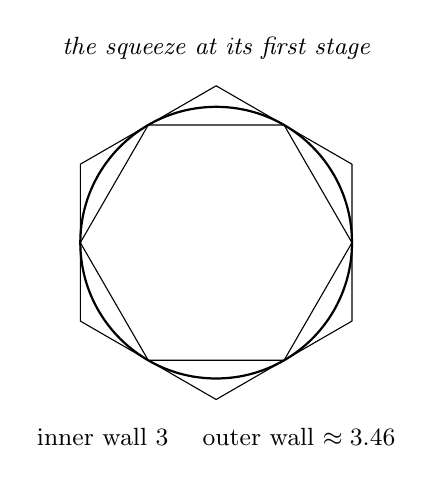
\begin{tikzpicture}[scale=1.15]
\draw[thick] (0,0) circle (1.5);
\draw (0:1.5) \foreach \a in {60,120,180,240,300} { -- (\a:1.5) } -- cycle;
\draw (30:1.7321) \foreach \a in {90,150,210,270,330} { -- (\a:1.7321) } -- cycle;
\node[font=\small] at (0,-2.15) {inner wall $3$ \quad outer wall $\approx 3.46$};
\node[font=\small\itshape] at (0,2.15) {the squeeze at its first stage};
\end{tikzpicture}
\caption{The circle imprisoned between its hexagons. Each doubling of sides is one
run of the squeeze: the walls at twelve, twenty-four, forty-eight, and ninety-six
sides march toward each other, never touching, and at ninety-six Archimedes quoted
his standing fences: $223/71$ and $22/7$.}
\end{figure}

And now the boundary of what the exhibit says, drawn exactly, because this book
draws its boundaries even where the reader's goodwill would excuse the blur. The
argument contains no circle. There is no formal object $\pi$ standing behind those
walls; "below the circle's true ratio" is not a theorem anywhere in this book,
because the argument has no curve to be below --- it has perimeter-counts, and the
bracket is on those measured convergents. Where the reader's mind supplies the
circle, the book supplies only polygons. The identification of the corridor's
occupant with the world's $\pi$ is the reader's step, taken outside the argument
--- and the reader takes it instantly and correctly, because the world's $\pi$
does lie inside the corridor. That is precisely what makes this a calibration: the
needle was pointed at known ground, and it landed where the known value lives. An
instrument does not earn trust by explaining itself; it earns trust by being
right where the answer is already known.

What the calibration licenses, and what it does not, in both directions:

\begin{fence}
The exhibit validates the method --- earned walls, proved order, an honest stop
--- and only the method. The circle's ratio does not vouch for the electron's
coupling: the flagship stands on its own three pins, and nothing in this section
is among them. And the guard runs both ways: if the squeeze were ever found
disordered, the calibration would die --- the flagship would not. Neither reading
is hostage to the other; they share a discipline, not a fate.
\end{fence}

The needle has now been seen moving on known ground. The next reading turns the
instrument to a weight --- the oldest hard measurement in physics, a balance in a
cellar, re-run as counts --- and the reader may bring to it the trust the exhibit
just earned.

\section{The balance}
% Node-map: D2 whole -- Cavendish told and re-run as counts (his row lands, Michell
% credited in a clause); the reading IS the ratio (G_device: numerator the one measured
% eighteen, denominator the mass product BY CONSTRUCTION); numerator-survives REFERENCED
% to Ch3, not re-told; the retirement honored IN the reading's statement, one clause;
% the MODEL-ROW falsifier (one named cancellation, cold-checked, no second pin);
% one-root reconnection in one clause. EXP-3 FORWARD-REF planted for Ch6.
% Gate: turn 522 (Ch5 S3, ~900 words).

In the last years of the eighteenth century, Henry Cavendish --- a man so afraid of
conversation that his servants were instructed to stay out of sight --- hung a
six-foot wooden arm from a wire in a closed shed, fixed a small lead ball to each
end, and brought two lead spheres of three hundred and fifty pounds each to rest a
few inches away. The gravitation between ball and sphere twisted the wire --- by a
breadth a hair would dwarf --- and he read the twist through a telescope from
outside the room, because the heat of his own body would have stirred the air enough
to drown the signal. The apparatus was inherited from John Michell, who died before
he could use it; the patience was Cavendish's own. What he measured, in the useful
shorthand, was the weight of the Earth, and the number his wire gave stands within
about one percent of today's. It is the oldest hard measurement in physics: a force
so weak that everything else in the world is noise against it, read by a wire, a
telescope, and a man who would not enter the room. His ledger row is earned here,
and the reader should notice what kind of experiment earns it: not a derivation ---
a trap, like the polygons; a patience, like the walk.

The instrument of this book has a cellar of its own, and the balance re-runs there
as counts. A source mass and a test mass: texts, whose mass is what mass has been
throughout --- the bulk of their elaboration, the cost the machine pays to work
them. An arm: the separation between stations, in the machine's own units of
distance. A deflection: the slip --- how much the count moves when the masses face
each other across the arm. Assemble them exactly as the shed did:

\begin{center}
$G_{\mathrm{device}} \;=\; \dfrac{\text{observed slip} \,\times\, \text{separation}^2}
{\text{source masses} \,\times\, \text{test mass} \,\times\, \text{arm}}$
\end{center}

--- every factor a count, the whole an exact ratio, nothing in it rounded and
nothing in it imported. This is the device's own $G$, and the naming follows the
book's standing discipline: $G_{\mathrm{device}}$, the balance's reading in the
instrument's frame, claiming kinship of architecture with the shed's number and
nothing more.

The reading is the ratio, and it is quoted only as the ratio. Its numerator is
eighteen --- the same eighteen earned at the first post of Chapter 4, spent here for
the third time, the one root answering at yet another post. Its denominator is the
mass product by construction, and "by construction" is the honor of the sentence:
the bare count of that denominator is never asserted anywhere in this book. The
reader knows from Chapter 3 exactly why --- the one count that ever moved lived
there, and it was retired, not repaired --- and this section does not re-tell that
story. It inherits the repair, and quotes the shape that survives it: eighteen,
over the bulk, the bulk dividing out.

The balance's falsifier is owed, and it is the cleanest in the book --- the model
row of the whole table. One named cancellation: the mass bulk divides out, and what
remains must be eighteen. That equality is machine-checked, cold, on every build of
the argument. If a cold run ever reads the surviving coupling as anything but
eighteen, this reading dies. There is no second pin and no partial credit; the
falsifier is one sentence long because the reading's architecture is one
cancellation deep. Scope as always: the falsifier guards the ratio --- the
asserted shape --- and nothing else.

One more thing was done to this family of readings, and the reader has not yet
been shown it. The book has twice mentioned a null fired at the flagship --- the
subtraction of two spellings that should leave nothing, and the residue that would
be signal if it survived. That firing is real, it is dated, and its target was
precisely the neighborhood of readings this chapter states. It is the next
chapter's story, and it is the reason the readings of this chapter can be stated
with a straight face: they have already survived the best shot the argument knew
how to take at them.

There remains one reading in the family --- the strangest one, where the
instrument's counts brush against mass and temperature and the book must fence
hardest --- and it closes this chapter next.

\section{The landing}
% Node-map: D4a CARRIED (the RECURSION SLIP named in full -- Ch4 S1's name-discipline
% promise paid with explicit back-reference; describe, describe the describing, once
% more: first difference ZERO proved, second difference MINUS TWENTY-ONE, negative,
% scale-invariant proved; the reading = mass as second difference = strain; the -21's
% DEFENSE is Ch6's property, one forward clause only). D4b FENCED + displayed (the
% chapter's hardest fence: the temperature is NOT in the device); Rindler/Unruh named
% as borrowed INTERPRETATION riding on carried machinery (F3 PARTIAL honored in
% advance). Annotation: Unruh + Rindler rows land (instruments-not-authorities).
% Chapter close: the four readings assembled, handed to Ch6.
% Gate: turn 523 (Ch5 S4, ~900 words).

Chapter 4 made a promise about a word. There would be, it said, a second quantity
wearing "slip" in its casual name --- a second difference, with a chapter of its own
--- and the two would share a word and nothing else. The promise comes due here. Meet
the recursion slip, and note what it is not: it is not the proximity slip of the
earn-site, not an inverse-square, not a displacement. It is what happens to cost when
description turns around and looks at itself.

The measurement is three sentences long. The machine describes a thing, and the
description costs what it costs. The machine then describes its describing --- the
tower of Chapter 3, climbed one story --- and that costs what it costs. Once more:
describe the describing of the describing. Three costs now stand in a column, and the
instrument takes differences. The first difference is zero --- exactly, provably:
climbing the first story of the tower costs nothing extra, the descriptions lie
level, and that levelness is a theorem of the record, not an observation that has
held so far. And the second difference is minus twenty-one.

The reader should sit with the sign before the magnitude. A tower that cost more at
every story would surprise no one --- bureaucracies work that way. A level first
story is elegant. But a negative second difference says the third description costs
less than the level ladder predicted: the tower, described deeply enough, begins to
carry some of its own weight. And the magnitude is not a trend fitted from noise; it
is exact, and it is scale-invariant --- proved, in the same for-every-load form as
the immunities of Chapter 3: multiply the whole apparatus by any bulk, and the minus
twenty-one stands unmoved. This is the landing: the instrument's mass-like reading
is the second difference of self-description --- a strain, a curvature in the tower
of descriptions --- and it is minus twenty-one, at every scale, with the first
difference provably zero beneath it.

What minus twenty-one is --- a genuine self-energy of the computation, or an
artifact of where the counting was cut --- is a question this section deliberately
does not argue, because the argument's answer was not produced by rhetoric. It was
produced by a kill test and a fired null, and both belong to the next chapter. This
section states the landing; the next defends it.

But one boundary belongs here, because it is this reading's own, and it is the
hardest fence in the chapter:

\begin{fence}
The instrument contains no temperature. The landing's full shape --- mass as the
second difference read against a temperature --- is stated in this book as a shape
and nothing more: the temperature it calls for is not measured by this device, not
derived by this argument, and no number for it appears anywhere in these pages.
Where the shape's denominator should be, the book writes a fence, and the fence is
the content.
\end{fence}

Why should a temperature enter at all? Here the book borrows, and credits what it
borrows. There is a reading of this instrument's situation in the geometry of
frames --- the language this chapter was announced in --- and it goes like this. An
observer who must accelerate merely to hold its place does not read the vacuum as
empty; by Unruh's result, acceleration reads as warmth, a temperature proper to the
frame. And this instrument is such an observer, in the borrowed picture: a machine
that must keep re-describing itself merely to stand still, climbing its tower not
as an excursion but as its condition, its frame the accelerated one that Rindler's
geometry describes. In that picture, the taper the record applies where a
measurement is cut off hard --- easing the edge rather than chopping it --- is
exactly the apodization an accelerated frame demands, lest the hard cut ring. The
machinery in that sentence is carried: the taper is real, the second difference is
real, both are in the record. The picture wrapped around them --- the warmth, the
frame, the why --- is interpretation, borrowed from Unruh and from Rindler, whose
ledger rows are earned here on the usual terms: instruments of understanding, not
authorities. The book finds the picture compelling and does not mistake compelling
for proved.

The chapter can now close on its full inventory, four readings in four postures.
The flagship: asserted, an interval with three pins under it. The exhibit:
calibrated, the needle watched landing where the world already knew the answer.
The balance: quoted, a ratio one cancellation deep. The landing: stated and
fenced, a minus twenty-one that is proved where it can be and fenced where it
cannot. Four readings, and one debt now overdue: twice this book has mentioned a
null fired at the heart of these numbers, and twice deferred it. The next chapter
pays. The bridge is built, the arms are balanced, and the shot is finally fired
on the page.
